\section{Introduction}
%

Recent advances in biomedical image analysis have assisted many pathologists and biologists to facilitate their researches \cite{Chen2016b,Ronneberger2015,Chen2016c,Lieman-Sifry2017,Paszke2016,Tseng2017,Sirinukunwattana2015b}.
An importance application is to obtain the accurate segmentation of specific membrane objects in a biomedical image, such as lumenal glands, synaptic vesicles and cells.
%
The morphological shape and spatial distribution of synaptic vesicles help the study of neural activities in different brain regions, while morphological statistics of lumenal glands are widely used for assessment of the malignancy degree of adenocarcinomas.
%
Conventionally, these crucial steps are performed by human experts, which are time-consuming and suffer from subjective factors.
Therefore, it is significantly demanded to improve the efficiency as well as the reliability with automatic segmentation methods.

\begin{figure}
    \begin{center}
        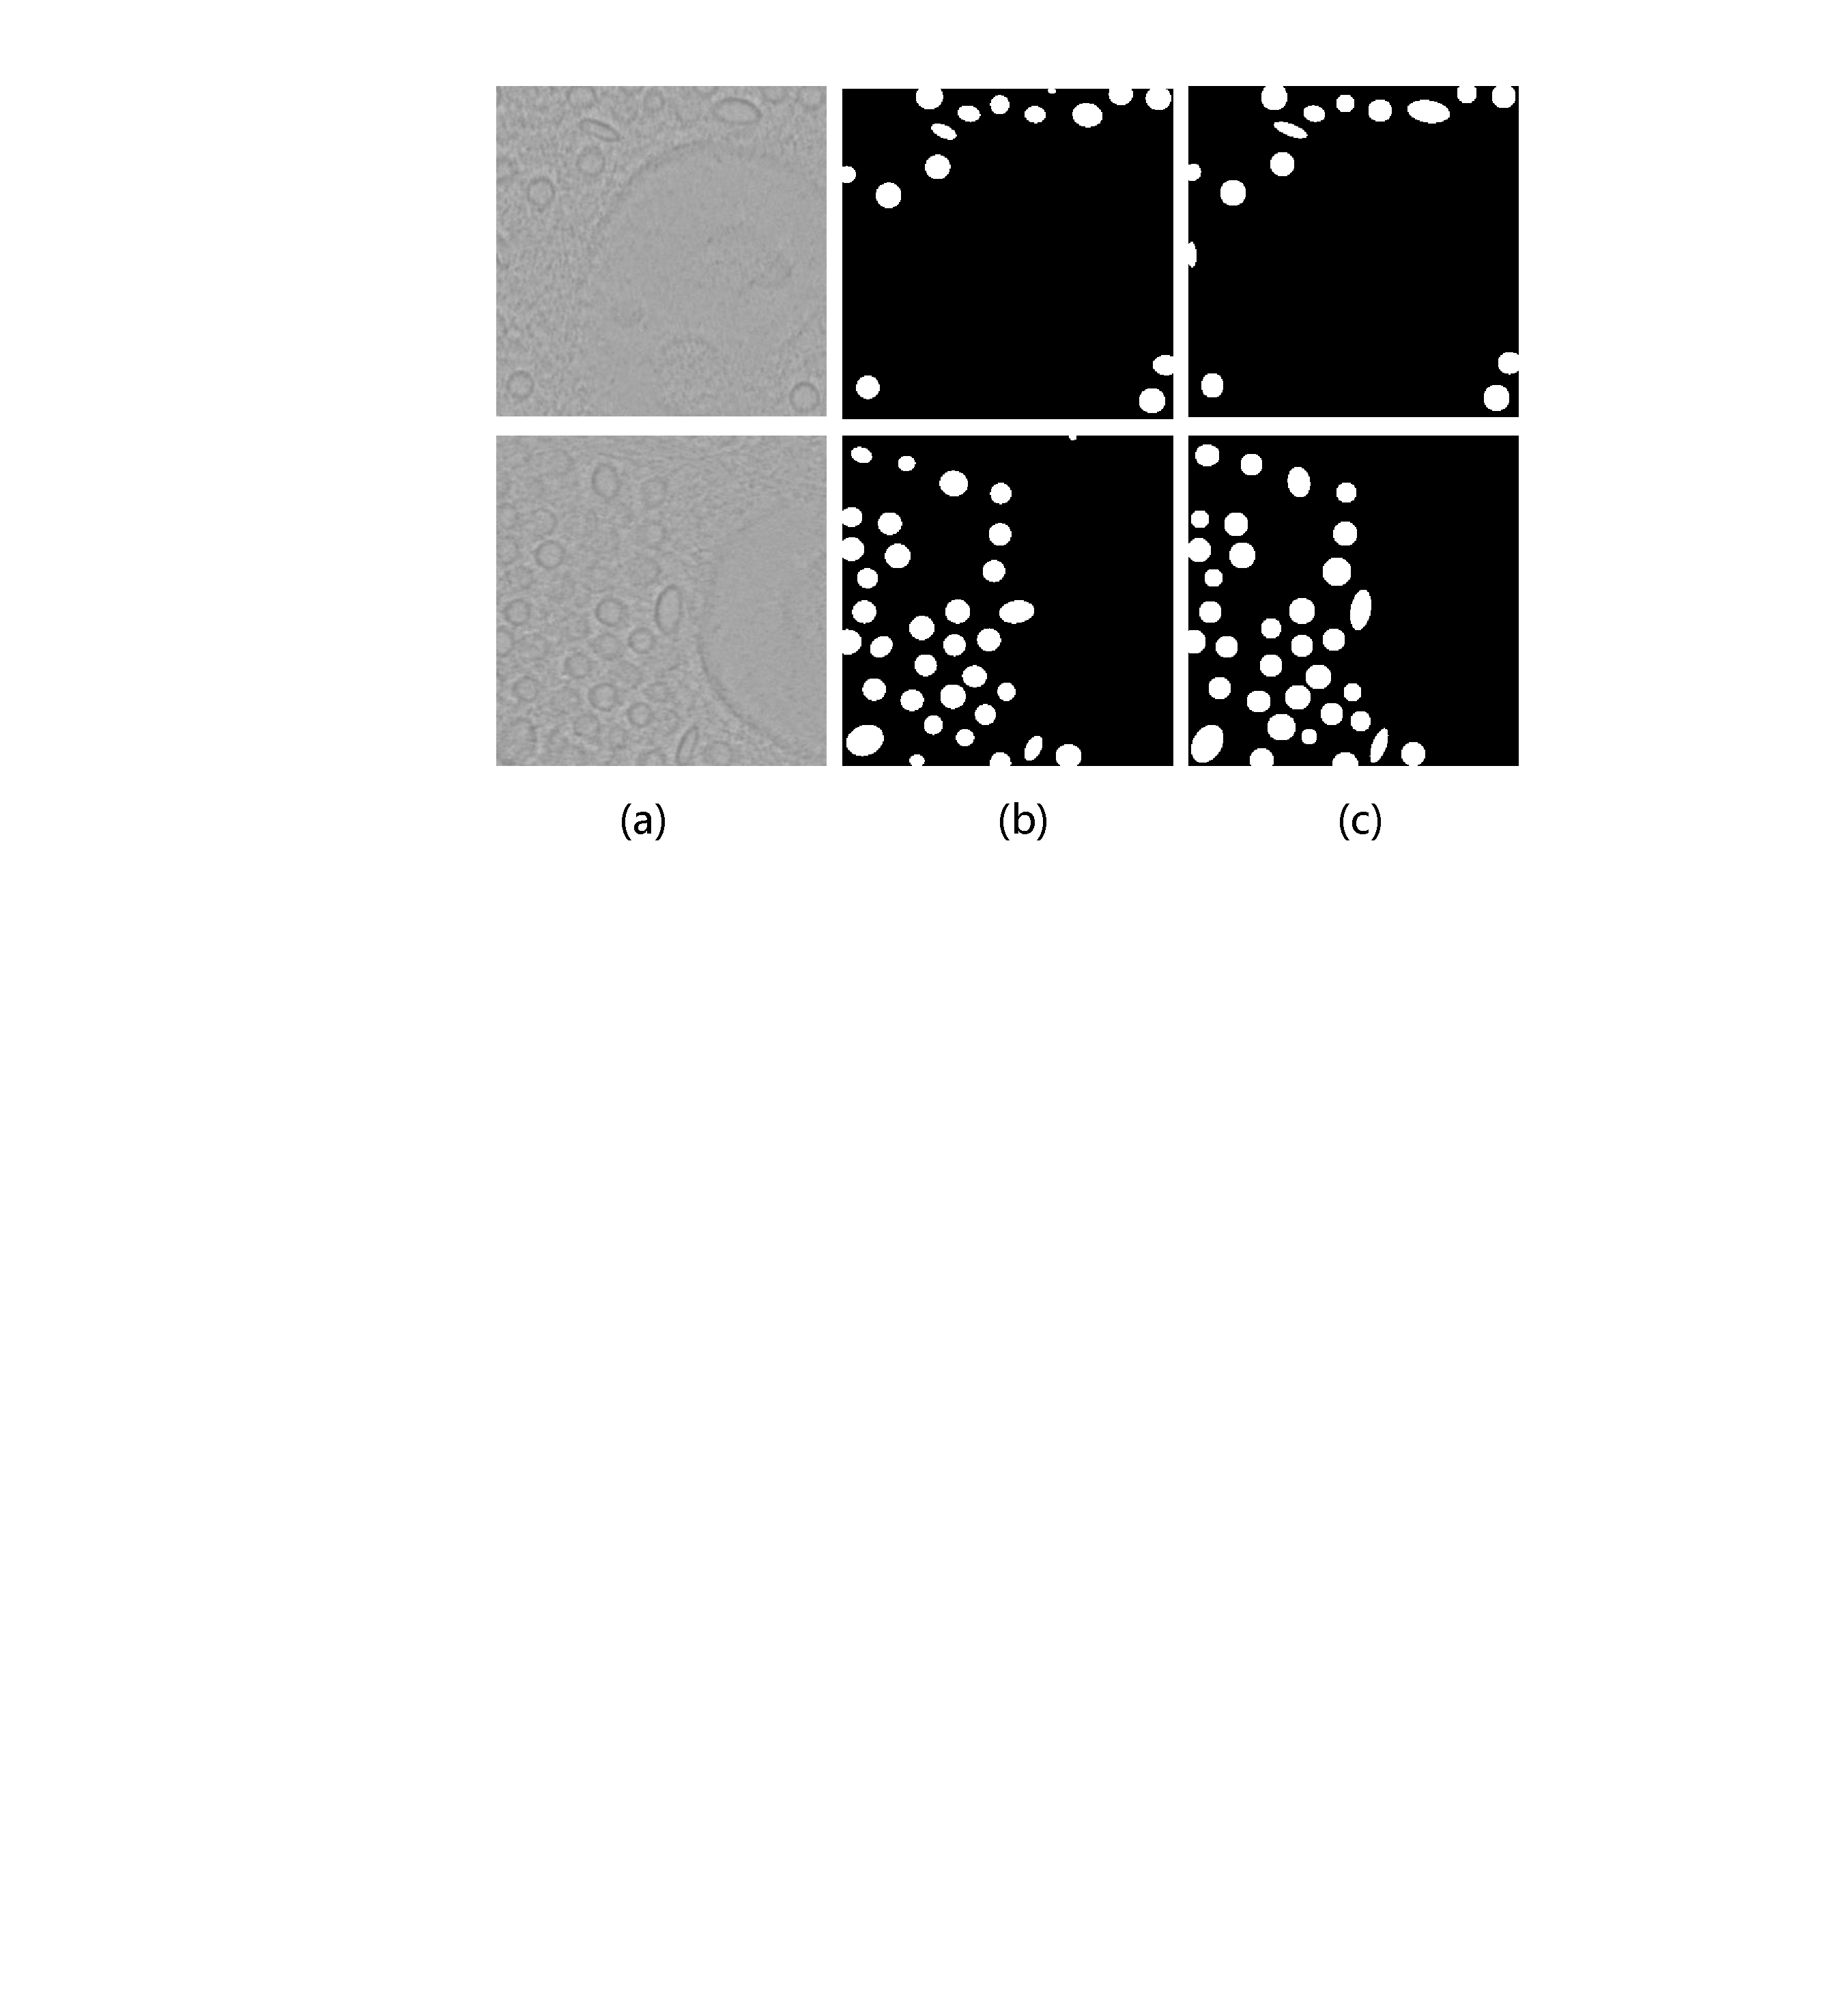
\includegraphics[width=3.3in]{figures/FigImg.pdf}
    \end{center}
    \caption{Examples of challenging biomedical segmentation: (a) biomedical image; (b) results from proposed DSAN by incorporating prior shape knowledge; (c) annotations by experts.}
    \label{fig:introImgs}
\end{figure}

However, it is non-trivial to automatically segment objects in biomedical images.
First, biomedical images are usually noisy and ambiguous caused by deficient imaging techniques, as shown in Figure~\ref{fig:introImgs} (a).
Second, the dense arrangement and blurry boundaries of objects in biomedical images make it difficult to separate adjacent objects. 
This is typically known as the touching problem in biomedical image segmentation.
%
Finally, it is challenging to incorporate prior shape knowledge about plausible objects to into the model, because of huge variation of some pathological objects~\cite{Sirinukunwattana2015b}.
%
\cxj{Does this paper use shape prior?}

%%%% Recent networks for image segmentation %%%%%%%%%%%%%
Recently, fully convolution network (FCN) networks have demonstrated tremendous progress in image segmentation \cite{Long2015a,Chen2016d,Dai2015,Zheng2015}.
The famous U-shaped deep network called U-net~\cite{Ronneberger2015} was proposed for biomedical image segmentation, which obtained great performance in solving touching problems.
%
The U-net used skip connections between contracting and expanding paths to supplement the lost information and further added weighting losses on boundary pixels for clear boundaries in segmentation.
%
Soon afterwards, DeepVentricle~\cite{Lieman-Sifry2017} uses the same padding instead of valid padding in cardiac segmentation.
\cxj{what do you mean by "the same padding"?}
%
A kU-net proposed in \cite{Chen2016c} employs multiple submodule FCNs to work on different image scales systematically.
%
Recently, DCAN~\cite{Chen2017} integrates complementary information of objects and contours in a multi-task learning framework to separate the clustered objects into individual ones, which obtains state-of-the-art performance.
Although these methods achieved promising results in their segmentation tasks, they may fail to achieve satisfying performance in more blurry images with denser and smaller objects.

\cxj{Add more explaination why the previous methods fail on denser and smaller objects? No training data or the scale is larger or something else? In another words, what is the difference between our problem and their problem? What is challenging here?}


In this paper, we propose a Deep Shape-Aware Network (DSAN) to segment dense objects by first inherently incorporating prior shape knowledge into network.
Similar with \cite{Chen2017,Ren2015,Li2016a,Chen2016,Bertasius2016}, we formulate the network as a multi-task learning framework by simultaneously predicting an objectness score map and several auxiliary maps for an input image.
Instead of contour probability as auxiliary \cite{Chen2017,Chen2016,Bertasius2016}, our DSAN learns the parameterized expression of each object shape, which emphasizes more on the overall shape.
%
Especially for each pixel, the DSAN simultaneously predicts an objectness score and a set of parameters, formulating the shape of a nearest object.
% which is inspired by \cite{Ren2015}.
The complementary information in auxiliary parameters can not only separate the objects into individual ones, but also optimize their shapes.

However, the object shapes cannot be parameterized uniformly and constrained strictly, due to the huge variation of object shapes in pathological cases.
%
Therefore, we select a best shape as constraint and employ a piecewise fusion strategy to generate the final segmentation masks, leveraging the shape regularization with boundary details in the image.
%which achieves a balance between regularization and unconstraint in segmented objects shape.
Furthermore, a novel split max pooling (SMP) is proposed to benefit both objectness scores and shape parameters by exploring the intrinsic correlation between them.
Besides, SMP is designed as a trainable layer, which can be trained end-to-end and easily extended to any multi-task networks.
With the above mentioned strategies, our DSAN can not only optimize the segmented shape of regular objects with prior shape knowledge, but also accommodates seriously deformable objects, as Figure~\ref{fig:introImgs} shows.

Overall, the contribution of this paper is three-fold:
\begin{enumerate}
	\item We first effectively incorporate shape constraints into deep neural networks. \cxj{Can we say we are first? compared with \cite{Ren2015}?}
	% for biomedical image segmentation.
	\item We propose a novel split max pooling for benefiting multi-task outputs together.
	\item Our framework is capable to handle the challenging biomedical segmentation tasks and achieves the state-of-the-art performance.
\end{enumerate}
